\chapter{Emission Modeling}
\label{ch:emissions}
% ##################################################################################################################

\hfill \textbf{Author:} Benjamin Kickhöfer

\begin{center} 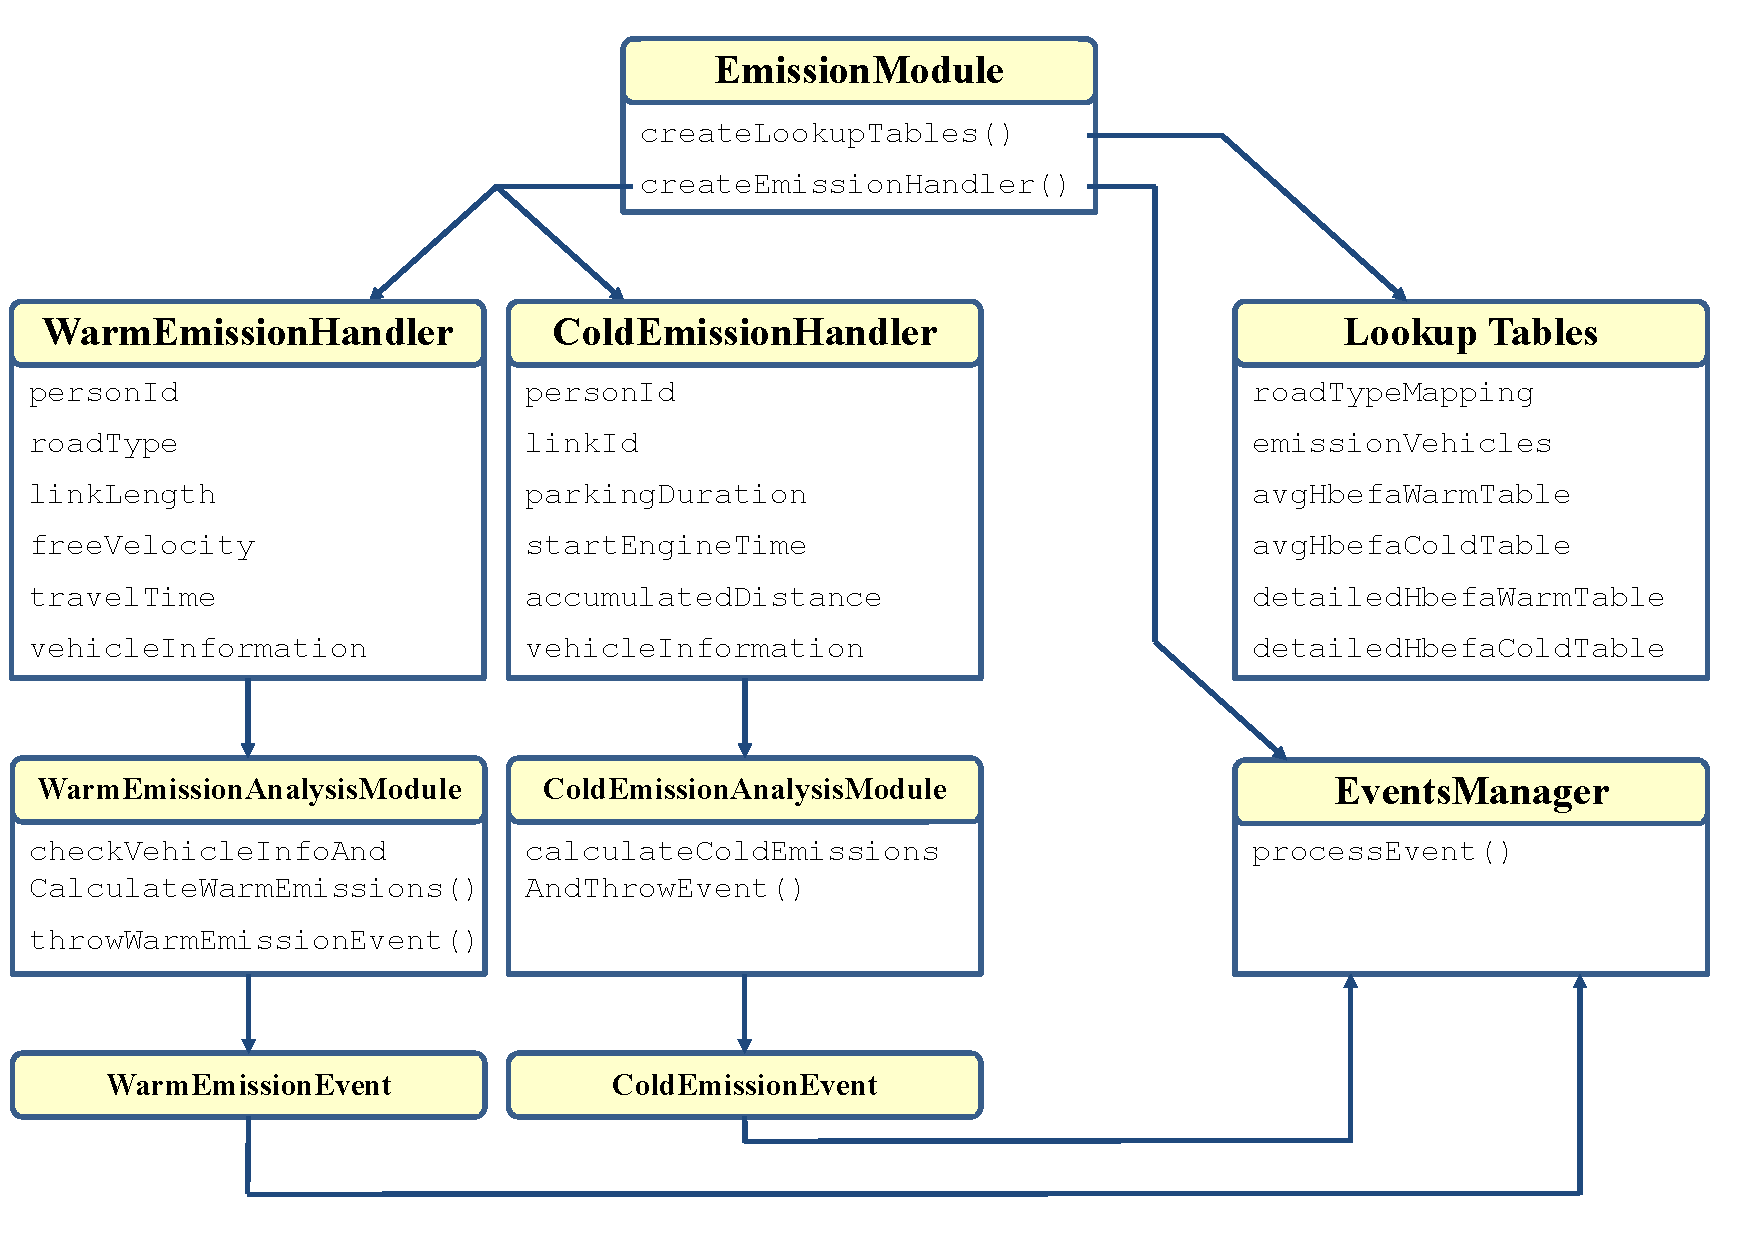
\includegraphics[width=0.4\textwidth, angle=0]{extending/figures/emissionToolOverview_pdfa.pdf} \end{center}

\createStandardInformation{emissions}{\lstinline|RunEmissionToolOnlineExample| class, \lstinline|RunEmissionToolOfflineExample| class}{emissions}
{\citet{HuelsmannEtAl_LAS_2011,KickhoeferEtAl_VanoutriveVerhetsel_2013,KickhoeferNagel2011MappingEmissions,KickhoeferEtAl_NSE_2013,HuelsmannEtAl_GerikeEtAl_2013,Kickhoefer_PhDThesis_2014,KickhoeferKern_MobilTUM_2014}}

% ##################################################################################################################
This chapter aims at presenting the emission modeling tool that has been developed and tested by \citet{HuelsmannEtAl_LAS_2011} and further improved by \citet{KickhoeferEtAl_VanoutriveVerhetsel_2013}. The text in this chapter is a slighted, updated version of the description of the emission modeling tool in \citet{Kickhoefer_PhDThesis_2014}.
%
The tool essentially calculates warm and cold-start exhaust emissions for private cars and freight vehicles by linking \glsentrytext{matsim} simulation output to the detailed database of the "\gls{hbefa}", which is available for many European countries.

The chapter is structured as follows:
%
Section ~\ref{ch:emissions:relatedWork} reviews other attempts in the literature to model transport related emissions. Section~\ref{ch:emissions:overview} presents an overview of the "\gls{emt}" and Section ~\ref{ch:emissions:structure} shows how the tool is embedded in \glsentrytext{matsim}'s software structure.

% ##################################################################################################################
\section{Integrated Approaches for Modeling Transport and Emissions}
\label{ch:emissions:relatedWork}
%
%\benjamin{This section maybe does not need to go into the MATSim book. Opinions?}
%
Over the last two decades, modeling transport related environmental 
externalities has gained more and more attention in transportation science.
%
For this reason, the following paragraphs shortly present some recent 
attempts in the area of exhaust emission modeling; additionally, they 
highlight differences to the \glsentrytext{emt} which will then be described in the 
subsequent sections.

\citet{CreutzigHe_TransResD_2009} and \citet{MichielsEtAl_TransResD_2012} use very 
aggregated figures to estimate air pollution in Beijing and whole of Belgium, 
respectively. Both approaches do not mention any particular underlying 
transport model. It seems that transport related emissions are based on
aggregated origin-destination matrices or aggregated demand functions. These 
two studies are on a very different level of aggregation than the \glsentrytext{emt} in 
this thesis, and a comparison does not seem very useful.

\citet{BeckxEtAl_EnvPlannB_2009} use a sophisticated 
activity-based model to simulate activity schedules for roughly 30\,\% of all 
households in the Netherlands. Traffic assignment for passenger cars is 
performed by using an aggregated `all-or-nothing' assignment approach, 
resulting in hourly aggregated traffic flows on the network. Based on the 
average speed for a trip, the \gls{mimosa} then 
calculates emission and fuel consumption rates, possibly dependent on vehicle 
category. The idea of using an activity-based model to simulate 
time-dependent emissions is similar to the \glsentrytext{emt}. In contrast to the 
latter, the underlying transport in \citet{BeckxEtAl_EnvPlannB_2009} 
does not account for congestion effects and different traffic states. 
Additionally, similar macroscopic emission models are typically unable to 
capture some of the microscopic behavior accurately 
\citep[see, e.g.,][]{AhnRakha_TransResD_2008}. 

\citet{HirschmannEtAl_ITSC_2010} link the microscopic traffic flow simulator "\gls{vissim}" with the instantaneous 
emission model "\gls{phem}"%
%
\footnote{
%
The model uses speed trajectories as input and was tested against the emission 
modeling tool of this thesis in a paper by 
\citet{HuelsmannEtAl_LAS_2011}.
%
}%
. At a first glance, this approach seems very promising, as it also builds the 
basis for the \glsentrytext{hbefa} database. In contrast to the \glsentrytext{emt}, it is not 
suitable for large-scale scenarios due to the computational complexity of 
\glsentrytext{vissim}.
%
In \citet{Kraschl-HirschmannEtAl_FISTS_2011}, the same authors attempt to 
develop a parametrization of fuel consumption based on average speeds of 
vehicles. Such parametrization could in the future be helpful to replace 
time-consuming lookups in large databases (e.g.,\,\glsentrytext{hbefa}). However, the 
model would need to allow for more input variables (e.g.,\,vehicle category, 
traffic state, etc.) and to provide more differentiated outputs such as 
different emission types.

In a similar study, \citet{SongEtAl_TRR_2012} couple \glsentrytext{vissim} with the emission modeling tool "\gls{moves}". They find 
that the \glsentrytext{vissim}-simulated vehicle-specific power distribution for 
passenger cars deviates significantly from the observed distribution. In 
consequence, the estimated emissions also contain significant errors. Here 
again, the proposed model can not be used for large-scale scenarios for the 
same reason as above. Additionally, it seems questionable whether such detailed 
modeling will become superior to less detailed models such as the \glsentrytext{emt} in 
this thesis.

\citet{WismansEtAl_TRB_2013} compare passenger car emission 
estimates of static and dynamic traffic assignment models. They claim that 
little research has been done in connecting macroscopic or meso-scopic dynamic 
traffic assignment models with emission models.
%
According to the authors, static assignment models predict congestion on the 
wrong locations and ignore spill-back effects. They argue that emission 
hotspots are, in consequence, also predicted at the wrong locations and/or 
with the wrong amplitude.
%
Therefore, they couple a static and a dynamic traffic assignment model with 
the exhaust emission model "\gls{artemis}". Large differences in air 
pollutant emissions are found, and hotspot locations differ.

\citet{HatzopoulouMiller_TransResD_2010} develop a methodology for 
calculating exhaust emissions, using \glsentrytext{matsim} as meso-scopic transport 
model. The approach is therefore fairly similar to the \glsentrytext{emt} of this thesis.
%
In contrast to that study, the \glsentrytext{emt} does not assume fixed exhaust 
emissions per time unit. It uses a more detailed calculation of emissions based 
on the two different traffic states "free flow" and "stop\&go". It is, thus, 
able to capture congestion effects that emerge additionally to the time spent 
in traffic jam. 
Furthermore, the \glsentrytext{emt} calculates exhaust emissions for passenger cars 
\emph{and} for trucks. Finally, since the methodology is based on \glsentrytext{hbefa}, 
it can be transferred to any scenario in Europe.

% ##################################################################################################################
\section{Emission Calculation}
\label{ch:emissions:overview}
%
Air pollution is caused by different contributions of road traffic:
%
Warm emissions are emitted while driving and are independent of the engine's temperature.
%
Cold-start emissions additionally occur during the warm-up phase and depend on the engine's temperature when the vehicle is started.
%
Warm emissions differ with respect to \emph{driving speed}, acceleration/deceleration, \emph{stop duration}, road gradient, and \emph{vehicle characteristics} that consist of vehicle type, fuel type, cubic capacity, and European Emission Standard Class \citep{AndreRapone_Atmos_2009}.
%
Cold emissions differ with respect to \emph{driving speed}, \emph{distance traveled}, \emph{parking time}, ambient temperature, and \emph{vehicle characteristics} \citep{WeilenmannEtAl_Atmos_2009}.

As of now, the emissions contribution to \glsentrytext{matsim} considers all differentiations from above which are marked in \emph{italic}. Road gradient and ambient temperature are not considered. The gradient is always assumed to be 0\,\%, and ambient temperatures are assumed to be \glsentrytext{hbefa} average.
%
Additionally to warm and cold-start emissions, evaporation and air conditioning emissions also result from road traffic. As of now, the latter are not considered in the emission modeling tool, because of the small contribution to the overall emission level.

The calculation of warm emissions is composed of two steps:
%
\begin{enumerate}
 \item Deriving \emph{kinematic characteristics} from the simulation
 \item Combining this information with vehicle characteristics in order to 
 extract emission factors from the \glsentrytext{hbefa} database
\end{enumerate}
%
In the first step, driving speed as well as stop duration (and possibly an 
approximation of acceleration/deceleration patterns) is captured by a 
mapping of \glsentrytext{matsim}'s dynamic traffic flows to \glsentrytext{hbefa} traffic states. 
These traffic states, namely "free flow", "heavy", "saturated", and "stop\&go", 
have been derived from typical driving cycles, i.e.,\,time-velocity profiles. 
A parametrization of these profiles led to the definition of these traffic 
states, which depend on speed limit, average speed, and road type. Thus, 
typical emission factors for a certain traffic state on a certain road segment 
can be looked up in the \glsentrytext{hbefa} database.
%
In \glsentrytext{matsim}, neither the location on a road segment nor the exact driving behavior of an agent is known (see Section~\ref{sec:trafficflowmodel}).
%
%\benjamin{Some pointer to the MATSim traffic flow model. Andi, can you do that?}
%
It is, however, rather straightforward to extract agent's travel times on the road segment which, thanks to the queuing model, also includes interactions with other agents and spillback effects.
%
Therefore, the average speed of an agent on a certain road segment is used to 
identify the corresponding \glsentrytext{hbefa} traffic states, and to assign emission 
factors to the vehicle. As of now, the emission modeling tool only considers 
the two traffic states free flow and stop\&go.%
% 
\footnote{
%
This simplification is due to the fact that the difference between the 
emission factors of the traffic states free flow, heavy, and saturated, are 
only marginal. In contrast to those traffic states, the emission factors for 
stop\&go are roughly twice as high.
%
}
%
Each road segment is divided into two parts representing these two 
traffic states. The distance $l_s$ that a car is driving in stop\&go traffic 
state is determined by the following equation:
%
\begin{equation}
l_s = \frac{l \ v_s  (v_f-v)}{v (v_f - v_s)} \ ,
\label{ch:emissions:eq:linkLengthStopGo}
\end{equation}
%
where $l$ is the link length in kilometers from the network, $v_s$ is the stop\&go speed in $km/h$ for the \glsentrytext{hbefa} road type, $v_f$ is the free flow speed in $km/h$ from the network, and $v=\frac{l}{t}$ is the average speed on the link for the vehicle, $t$ being the link travel time of the vehicle in the simulation. For the derivation of Equation~\ref{ch:emissions:eq:linkLengthStopGo}, please refer to \citet{Kickhoefer_PhDThesis_2014}. The distance that the car is driving in free flow traffic state is then simply the remaining link length $l_f = l - l_s$.
%
The interpretation of this approach is the following:
%
Cars drive in free flow until they have to wait in a queue. Only in the queue, stop\&go traffic state applies. According to the \glsentrytext{matsim} queue model presented in Section~\ref{sec:trafficflowmodel}
%
%\benjamin{Some pointer to the MATSim traffic flow model. Andi, can you do that?}
%
, a queue emerges if demand exceeds capacity of a road segment which can also result in spill-back effects on upstream road segments. The length of the queue is, thus, approximated by Equation~\ref{ch:emissions:eq:linkLengthStopGo}, where the average speed $v$ on a link is the only exogenous variable.

For the second step, agent-specific vehicle attributes are needed. They are 
usually obtained from survey data during the initial population 
synthesis. The vehicle attributes typically comprise vehicle type, age, cubic 
capacity and fuel type. As \glsentrytext{matsim} keeps socio-demographic information throughout 
the simulation process, it can be used at any time for the necessary lookup in the 
detailed \glsentrytext{hbefa} database. Additionally, the emission modeling tool 
is designed in such way that fleet averages are used, whenever no detailed 
vehicle information is available.

The calculation of cold-start emissions is again composed of two steps:
%
\begin{enumerate}
 \item Deriving \emph{parking duration} and \emph{accumulated distance} 
 from the simulation
 \item Combining this information with vehicle characteristics in order to 
 extract emission factors from the \glsentrytext{hbefa} database%
 % 
 \footnote{
 %
 Please note that \glsentrytext{hbefa} provides cold-start emission factors only for 
 passenger cars. Freight traffic therefore only produces cold-start emissions 
 of passenger cars.
 %
 }
 %
\end{enumerate}
%
Parking duration refers to the time a vehicle is not moved \emph{before} 
cold-start emissions are produced. It is calculated by subtracting an 
activity's start time from the same activity's end time and by checking if the 
trip to and from the activity is performed by car. Emission factors in 
\gls{hbefa} 
are differentiated by parking duration in one hour time steps from 1\,hour to 
12\,hours. After 12\,hours, the vehicle is assumed to have fully cooled down.
%
The accumulated distance refers to the distance a vehicle travels \emph{after} 
a cold start. According to \glsentrytext{hbefa}, there are different cold-start 
emissions for short trips smaller than 1\,kilometer and and for longer trips grater or equal than 1\,kilometer.
%
In reality, cold-start emissions are emitted along the route after a cold start;
as of now, the emission modeling tool maps the emissions of the short trip to the road
segment where the engine is started, and, if applicable, additional emissions
to the road segment where the accumulated distance exceeds the first kilometer.
%
Overall, cold-start emission factors increase with parking duration and 
accumulated distance. Additionally, they depend on vehicle attributes. The 
lookup for this information is identical to the one described for warm 
emissions.

In order to further process the warm and cold-start emissions, so-called 
\emph{emission events} are generated during the simulation in a separate 
events stream. The definition of emission events follows the \glsentrytext{matsim} 
framework that uses events for storing disaggregated information in 
\glsentrytext{xml} format. The following section will now provide more information 
on the software structure of the emission tool.

% ##################################################################################################################
\section{Software Structure}
\label{ch:emissions:structure}
The information in this section refers to code that can be found in the 
\glsentrytext{matsim} repository.%
%
\footnote{
%
The exact location at the time of writing is 
\url{https://svn.code.sf.net/p/matsim/source/contrib/trunk/emissions}.
%
}
In the following, the software structure of the \glsentrytext{emt} at 
revision 30\,058 is described. For information on how to use the tool, please 
refer to \lstinline|package-info.java| in the corresponding package.%
%
\footnote{
%
This information can also be accessed via the javadoc page for the emissions contribution; see \url{http://matsim.org/javadoc}.
%
}
%

Figure~\ref{ch:emissions:fig:emissionTool} shows the simplified software structure of the emission modeling tool. The core of the tool is the \lstinline|EmissionModule| which needs to be created before the simulation starts. Additionally, there are two public methods that need to be called: \lstinline|createLookupTables()| and \lstinline|createEmissionHandler()|.
%
% ------------
\createfigure%
{Software structure of the emission modeling tool}%
{Software structure of the emission modeling tool}%
{\label{ch:emissions:fig:emissionTool}}%
{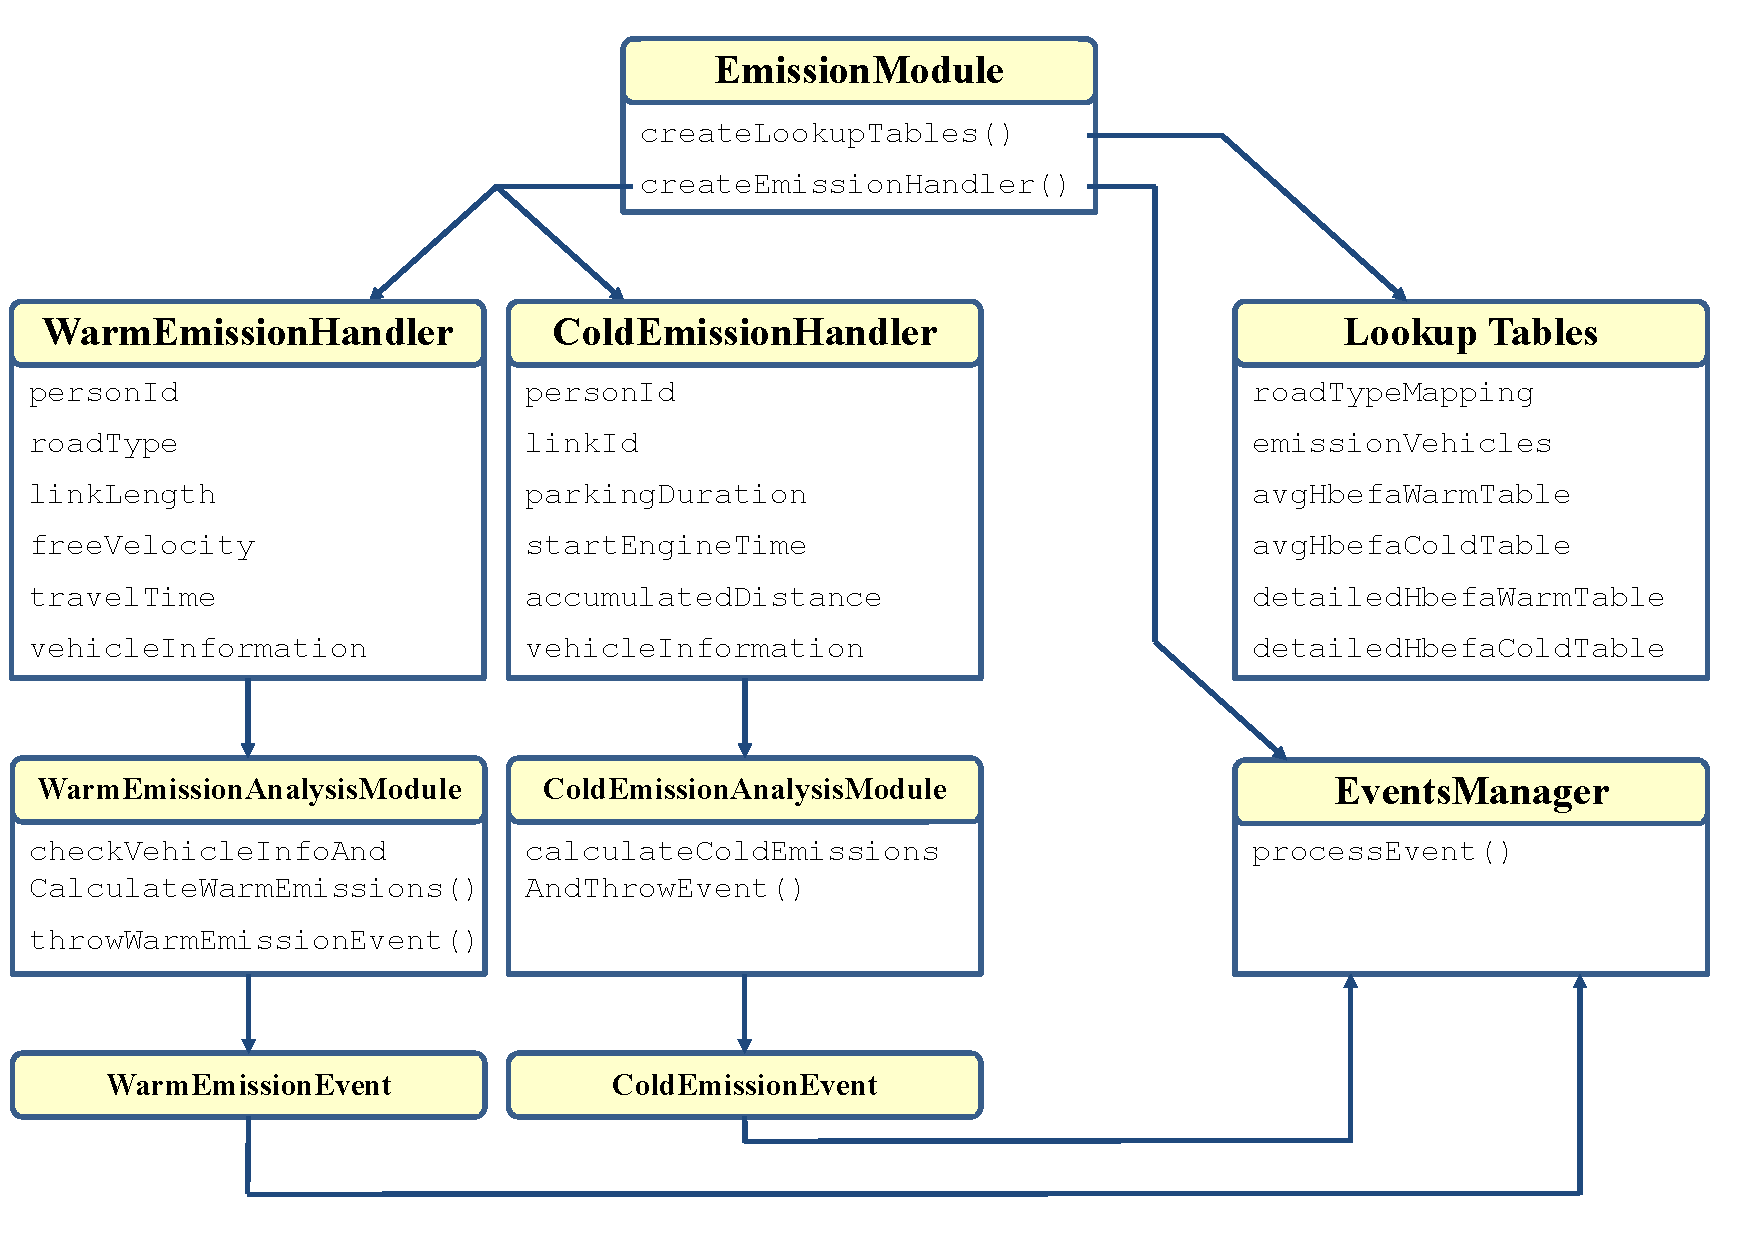
\includegraphics[width=0.99\textwidth, angle=0]{extending/figures/emissionToolOverview_pdfa.pdf}}%
{}

% ------------
The former creates lookup tables from input data that has to be exported from the \glsentrytext{hbefa} database. The path to these input files can be configured in the \lstinline|EmissionsConfigGroup|. Mandatory input are files for the creation of \lstinline|roadTypeMapping|, \lstinline|emissionVehicles|, \lstinline|avgHbefaWarmTable|, and \lstinline|avgHbefa-Cold-Table|.
%
The first lookup table maps road types from the \glsentrytext{matsim} network to \glsentrytext{hbefa} road types. For this mapping, it is necessary to classify the network road types into \glsentrytext{hbefa} categories; this requires some transport engineering knowledge.
%
The second lookup table defines the vehicle attributes of every person in the population. It should therefore be generated during the population synthesis process. If no detailed information is available, the vehicle lookup table still needs to specify whether the vehicle is a car or a truck. The current implementation uses the \glsentrytext{matsim} vehicle interface 
\lstinline|Vehicles| as container for storing the relevant data in \lstinline|VehicleType|.%
%
\footnote{
%
Please note that vehicle information provided to the \lstinline|EmissionModule| is \emph{only} used for storing data on individual vehicle characteristics and other information will be omitted by the simulation.
%
}
%
The last two mandatory lookup tables (\lstinline|avgHbefaWarmTable| and \lstinline|avgHbefaColdTable|) provide warm and cold emission factors in $g/km$, respectively. The data is stored using a unique key. For the construction of this key, information from \lstinline|roadTypeMapping| and \lstinline|emissionVehicles| is needed as well as information derived from the simulation as described in Section~\ref{ch:emissions:overview}.
%
The latter information is depicted in Figure~\ref{ch:emissions:fig:emissionTool} as variables of the two classes \lstinline|WarmEmissionHandler| and \lstinline|ColdEmissionHandler|. These two handlers implement several \glsentrytext{matsim} \lstinline|EventHandler| interfaces in order to extract the necessary information from the simulation. After gathering this information, the \lstinline|WarmEmissionHandler| asks its \lstinline|WarmEmissionAnalysisModule| to reconstruct the key and look up the emission factors in the respective table. Similarly, the \lstinline|ColdEmissionHandler| asks the \lstinline|ColdEmissionAnalysisModule|. These analysis modules then create \lstinline|Warm/ColdEmissionEvents| which follow the \glsentrytext{matsim} \lstinline|Event| interface definition. Finally, the resulting events stream is written in a joint emission events file by a separate \lstinline|EventsManager|.

For the calculation of emissions that depend on agent-specific vehicle characteristics, \lstinline|emissionVehicles| must contain that specific information, the corresponding flag in the \lstinline|EmissionsConfigGroup| needs to be switched on, and detailed emission factor tables additionally need to be exported from \glsentrytext{hbefa} and provided to the \lstinline|EmissionModule| with two additional input files: \lstinline|detailed\-HbefaWarmTable| and \lstinline|detailedHbefaColdTable|.

% ##################################################################################################################
